% SPDX-License-Identifier: CC-BY-SA-4.0
% Author: Matthieu Perrin
% Part: 
% Section: 
% Sub-section: 
% Frame: 

\begingroup

\begin{frame}{Grammaire française}

  Une grammaire est une collection de règles grammaticales du type : 
  \begin{itemize}
  \item \og Une phrase est formée d'un sujet, et d'un groupe verbal \fg
    $$ \mathit{Phrase} \rightarrow \mathit{Sujet}~\mathit{GV}$$
  \end{itemize}

  \begin{center}
    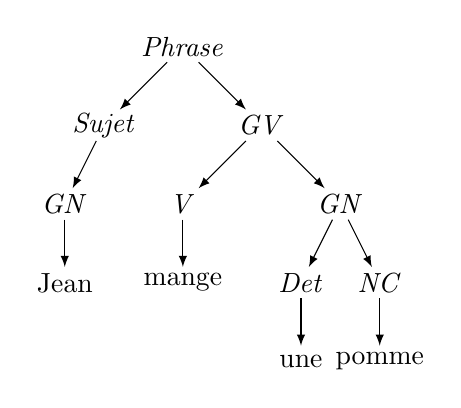
\begin{tikzpicture}
      \draw (5.0,10) node {$\mathit{Phrase}$};
      \draw (4.0,9 ) node {$\mathit{Sujet}$};
      \draw (6.0,9 ) node {$\mathit{GV}$};
      \draw (3.5,8 ) node {$\mathit{GN}$};
      \draw (5.0,8 ) node {$\mathit{V}$};
      \draw (7.0,8 ) node {$\mathit{GN}$};
      \draw (3.5,7 ) node {Jean};
      \draw (5.0,7 ) node {mange};
      \draw (6.5,7 ) node {$\mathit{Det}$};
      \draw (7.5,7 ) node {$\mathit{NC}$};
      \draw (6.5,6 ) node {une};
      \draw (7.5,6 ) node {pomme};

      \draw[-latex] (4.8,9.8) -- (4.2,9.2);
      \draw[-latex] (5.2,9.8) -- (5.8,9.2);
      \draw[-latex] (3.9,8.8) -- (3.6,8.2);
      \draw[-latex] (5.8,8.8) -- (5.2,8.2);
      \draw[-latex] (6.2,8.8) -- (6.8,8.2);
      \draw[-latex] (3.5,7.8) -- (3.5,7.2);
      \draw[-latex] (5.0,7.8) -- (5.0,7.2);
      \draw[-latex] (6.9,7.8) -- (6.6,7.2);
      \draw[-latex] (7.1,7.8) -- (7.4,7.2);
      \draw[-latex] (6.5,6.8) -- (6.5,6.2);
      \draw[-latex] (7.5,6.8) -- (7.5,6.2);
    \end{tikzpicture}
  \end{center}
  
  Les grammaires décrivent des mots et des langages par \structure{réécriture}.\\
  À la différence des définitions rationnelles, elles autorisent la \structure{récursivité}. 
\end{frame}
\endgroup
